\documentclass[10pt,a4paper,twoside]{report}
\usepackage[utf8x]{inputenc}
\usepackage[french]{babel}
\usepackage[T1]{fontenc}
\usepackage{amsmath}
\usepackage{amsfonts}
\usepackage{amssymb}
\usepackage{graphicx}
\usepackage{listings}
\usepackage[left=2cm,right=2cm,top=2cm,bottom=2cm]{geometry}
\usepackage{natbib}


\usepackage[x11names]{xcolor}
\usepackage{booktabs}


\usepackage[%
 pdfstartview=FitH,%
 bookmarks=true,%
 bookmarksopen=true,%
 breaklinks=true,%
 colorlinks=true,%
 linkcolor=blue,anchorcolor=blue,%
 citecolor=blue,filecolor=blue,%
 menucolor=blue,%
 urlcolor=blue]{hyperref}

\lstdefinestyle{mystyle}{
breakatwhitespace=false,
    commentstyle=\color{gray},
    keywordstyle=\color{Green4},
    numberstyle=\footnotesize\color{gray},
    stringstyle=\color{purple},
    identifierstyle=\color{SteelBlue4},
    basicstyle=\ttfamily\small,
    numbers=left,
    keepspaces=false,
    numbers=left,
    showspaces=false,
    showstringspaces=true,
    xleftmargin=20pt,
    }
\lstset{style=mystyle}

% \begin{lstlisting}[language=python]
% \end{lstlisting}

\begin{document}


\begin{titlepage}
\vspace*{5cm}
\begin{flushright}
{\Huge\sf OpenPattern}
\vspace*{1cm}

\begin{center}
\includegraphics[height=7cm]{/home/metivier/Nextcloud/Personnel/couture/Sewing/Daniel_bw.jpg}
\includegraphics[height=7cm]{/home/metivier/Nextcloud/Personnel/couture/Sewing/Sophie_bw.jpg}
\includegraphics[height=7cm]{/home/metivier/Nextcloud/Personnel/couture/Sewing/Greg_bw.jpg}
\end{center}

\vspace*{1cm}
{\Large\sf F. Métivier}\\
\vspace*{1cm}
{\sf\today}
\end{flushright}


\end{titlepage}
% \maketitle
\pagestyle{headings}
\tableofcontents


\chapter{Introduction}

\section{What is it}
OpenPattern  est une librairie python, orientée objet,  dont l'objectif est de permettre le tracé de patrons, en particulier de vêtements, à l'échelle 1:1 et leur sauvegarde au format pdf ou svg. Les patrons ainsi construits peuvent soit être directement imprimés pour utilisation soit être repris dans un logiciel de dessin comme Inkscape ou Illustrator.
OpenPattern offre la possibilité de créer des patrons «from scratch», d'utiliser des librairies de patrons existants (patrons de bases notamment) et de les reprendre pour les adapter et les transformer.

Les patrons peuvent être construits sur-mesures à partir d'un ensemble de mesures effectuées sur le corps d'une personne particulière (j'ai créé OpenPattern pour dessiner des vêtements pour ma famille), ou construits à partir de mesures de prêt à porter classique.

Les sources que j'ai utilisées pour tracer les patrons proviennent d'ouvrage de patronnages classiques. Ces ouvrages, destinés au couturiers amateurs ou aux étudiants d'écoles de modes, décrivent les techniques de réalisation de ce que l'on nomme la coupe à plat c'est-à-dire  la manière de projeter et tracer sur un plan (le papier puis le tissus) une forme géométrique 3D (le vêtement fini).

J'ai utilisé les ouvrages de quatre auteurs ou autrices principaux.
En premier lieu j'ai utilisé les quatre tomes de la série \textit{Le modélisme de mode} de Teresa Gilewska pour la femme et pour l'homme\cite{Gilewska1,Gilewska2,Gilewska4,Gilewska5}. J'ai aussi eu recours à deux tomes des ouvrages d'Antonnio Donnanno pour femme et homme également \cite{Donnanno2005,Donnanno2016}. Pour les enfants j'ai utilisé le tome correspondant de Jacqueline Chiappetta  \cite{Chiappetta1999} (mon préféré). Enfin pour l'homme j'ai aussi eu recours au livre de  Claire Wargnier sur le vestiaire masculin \cite{wargnier2012}. Ces ouvrages sont tous rédigés de façon similaire. Ils exposent, en procédant pas à pas, les techniques empiriques de tracé d'un body, d'un pantalon, d'une chemise etc.

la création d'un patron est donc une suite d'instruction comme «tracer un segment AB de longueur égale au 1/4 du tour de bassin» ou encore «ajouter une pince de 1.5 cm de 9cm de profondeur entre les points F1 et H» etc...
OpenPattern reprend de façon quasi litérale ces techniques et leur principe de construction en les adaptant quand cela se révèle nécessaire\footnote{Ces ouvrages présentent parfois des coquilles ou des imprécisions qui  sont probablement corrigées par leurs auteurs quand elles ou ils enseignent.}.

Contrairement aux logiciels payant ou gratuits de patronnage le parti-pris ici est de créer  un patron au moyen d'un script, c'est à dire d'une série d'instructions, et non de le dessiner avec un interface utilisateurs graphiques. cela peut sembler rébarbatif au premier abord mais cela offre toute la souplesse d'un langage de programmation comme python.

\section{How is it organized}

OpenPattern est organisée autour de classes qui héritent les unes des autres. Cette structure présente l'avantage de coller aux techniques de coupe. En effet une chemise, une veste ou un gilet sont des adaptations d'un body, une robe dérive de l'assemblage d'une jupe et d'un body, enfin les jupes et les pantalons dérivent de formes génériques dites de bases (jupe de base, pantalon de base).

OpenPattern présente pour l'instant deux niveaux d'héritage.
\begin{itemize}
\item La classe parente Pattern : C'est la classe générale qui définit ce qu'est un patron et les méthodes permettant de le dessiner et de le manipuler
\item Les classes de bases dérivées de Pattern: Basic\_Bodice, Basic\_Trousers, Cuffs, Collars
\item Les classes dérivées des classes de base: shirt, pyjamas qui héritent de Basic\_Bodice ou de Basic\_Trousers. \item Enfin les patrons font appels à une classe Point qui permet de définir un point de patronnage avec sa position et ses propriétés. Cette classe redéfinit les opérations d'addition et offre diverses manipulations  comme la rotation. L'intérêt ici est d'avoir un objet flexible qui permette de partir d'un patron de base et de l'altérer.
\end{itemize}

Pour dessiner un patron il faut
\begin{enumerate}
\item créer une instance de la classe correspondante,
\item appeler différentes méthodes d'altération ou de modification,
\item dessiner et, au besoin, sauvegarder le patron.
\end{enumerate}

Le dessin du patron peut aussi  directement se faire à partir des classes Pattern et Point comme nous allons le voir dans la suite de ce document.

\chapter{Tutoriel}



\section{Introduction: le patron de base}

Ce tutoriel montre comment utiliser les classes permettant de tracer des patrons complets à partir de mesures moyennes (un 38 français par exemple) ou à partir de mesures prises sur la personne de votre choix.
Différentes classes permettent de faire ce premier travail, le plus difficile parfois, qui consiste à tracer une base de patron:  base de pantalon, base de jupes, base de buste et de manche. À partir de ces patrons  il est alors  possible soit d'utiliser directement la base (pour une jupe droite ou un pantalon basique par exemple) soit de les «altérer» ou «transformer».

Le script suivant montre le principe d'utilisation de la librairie OpenPattern en prenant l'exemple d'un Body.  Nous allons tracer et enregistrer un patron de Body de femme sans pinces en 36 (taille française) selon la méthode de Gilewska.

\begin{lstlisting}[language=python]
import matplotlib.pyplot as plt
import OpenPattern as OP

# Creation de l'instance
p = OP.Basic_Bodice(pname = "W36G", gender = 'w', style = 'Gilewska')

# appel de la fonction de dessin
p.draw_bodice({"Pattern":"Bodice without dart"}, save=True)

plt.show()
\end{lstlisting}

C'est simple non ? On obtient alors la figure~\ref{fig:bodice_WG36} enregistrée par defaut à l'échelle 1:1 dans un fichier pdf. Les différentes options sont passées dans les arguments des différentes méthodes de classe (\texttt{draw\_bodice}) ou lors des instanciations de classe (\texttt{Basic\_Bodice} dans cet exemple).



\begin{figure}[hbtp]
\centering
\includegraphics[width=0.7\linewidth]{../patterns/Gilewska_Bodice_withour_dart_36.pdf}
\caption{Buste de base de femme, taille 36, sans pinces, d'après Gilweska.}
\label{fig:bodice_WG36}
\end{figure}

La liste des bases actuellement disponibles est donnée table \ref{tab:basic_classes}. Nous allons dans la suite voir en détail chacune des bases et leurs options.


\begin{table}[h]
\begin{center}
\begin{tabular}{llll} \hline
\multicolumn{4}{c}{\textbf{Body}}\\
Style & Femmes & Hommes & Enfants \\ \hline
 Chiappetta & & & 10-16\\
 Donnanno & x & x &\\
 Gilewska & x & x &\\ \hline
 \multicolumn{4}{c}{\textbf{Manche}}\\
 Style & Femmes & Hommes & Enfants \\ \hline
  Chiappetta & & & \\
  Donnanno &  &  &\\
  Gilewska & x & x &\\ \hline
 \multicolumn{4}{c}{\textbf{Pantalon}}\\
 Style & Femmes & Hommes & Enfants \\ \hline
 Chiappetta & & & \\
 Donnanno & x & x &\\
 Gilewska & & &\\ \hline
 \multicolumn{4}{c}{\textbf{Jupe}}\\
 Style & Femmes & Hommes & Enfants \\ \hline
 Chiappetta & & & 2-16 \\
 Donnanno & x &  &\\
 Gilewska & & &\\ \hline
\end{tabular}
\end{center}
\label{tab:basic_classes}
\caption{Classes de bases et styles implémantés. Les manches font partie de la classe body car elles sont calculées à partir des profondeurs d'emmanchure mesurées sur les body.}
\end{table}
% À vérifier mais il y a des variations avant 10 ans et il faudra probablement le reprendre car j'ai voulu dans un mauvais souci d'harmonisation inverser le dos et le devant.}.



\section{La jupe}

Le script suivant montre comment créer une jupe de base (ou jupe crayon ou encore fuseau ou pencil en anglais) et la figure~\ref{fig:pencil} montre le résultat.

\begin{lstlisting}[language=python]
import OpenPattern as OP
p = OP.Basic_Skirt(pname="W6C", style='Chiappetta', gender = 'G', ease=8, curves=False)
p.draw()
\end{lstlisting}

\begin{figure}[h]
\begin{center}
\includegraphics[width=0.7\textwidth]{../patterns/Donnanno_myPattern_W40D_FullSize}
\end{center}
\label{fig:pencil}
\caption{Jupe de base ou jupe crayon ou pencil skirt. Modèle d'après Donnanno, taille 40 italienne.}
\end{figure}



Les arguments à l'instanciation de la classe sont

\begin{tabular}{lllc}\\
Argument & type &  Définition & valeur par défaut\\ \hline
pname & str & code de la taille& W6C\\
style & str & modèle utilisé& Chiappetta\\
gender & str & genre & G\\
ease & int ou float & aisance à appliquer au patron& 8\\
curves & boolean & doit on oui ou non dessiner une taille courbe& False\\
\end{tabular}

Chez Donnanno la jupe crayon est symmétrique alors que chez Gilewska elle est légèrement asymétrique avec un demi-devant plus large de 1cm que le demi-dos. Pour Donnanno cette asymmétrie est une transformation et on la retrouvera dans la jupe «shifted-side-seams». Chez Chiappetta la jupe crayon fille est symmétrique quel que soit l'âge. 

\section{Le pantalon}

\section{Le body}

\begin{lstlisting}[language=python]
Basic_Bodice(pname="M44G", gender='m', style='Gilewska', age=12,\
  ease=8, hip=True):

draw_bodice(self, dic = {"Pattern":"Dartless bodice"}, save = False,\
  fname = None, paper='FullSize'):

\end{lstlisting}

Les figures~\ref{fig:bodice_DW36}, \ref{fig:bodice_MG36} et \ref{fig:CB14} montrent quelques exemples de body obtenus pour différents styles.


\begin{figure}[hbtp]
\centering
\includegraphics[width=0.7\linewidth]{../patterns/Donnanno_Bodice_withour_dart_36.pdf}
\caption{Buste de base de femme, taille 36, sans pinces, d'après Donnanno.}
\label{fig:bodice_DW36}
\end{figure}

\begin{figure}[hbtp]
\centering
\includegraphics[width=0.7\linewidth]{../patterns/Gilewska_Bodice_withour_dart_M36.pdf}
\caption{Buste de base d'homme, taille 36, sans pinces, d'après Gilewska}
\label{fig:bodice_MG36}
\end{figure}

\begin{figure}[hbtp]
\centering
\includegraphics[width=0.7\linewidth]{../patterns/Chiappetta_bodice_G14.pdf}
\caption{Buste de base de garçon, 14 ans, sans pince, d'après Chiappetta.}
\label{fig:CB14}
\end{figure}


% \begin{lstlisting}[language=python]
% Basic_Bodice(pname="M44G", gender='m', style='Gilewska', age=12,\
%   ease=8, hip=True)
% Basic_Trousers(pname="M44D", gender='m', style='Donnanno',darts= True)
% Basic_Skirt(pname="W6C", style='Chiappetta', gender = 'G', ease=8)
% \end{lstlisting}

\section{Les Transformations}


Aux trois classes de bases s'ajoutent des classes accessoires pour les manchettes et les colles
et en cours (et que je ne mets pas) des classes pour les gilets et pour les chemises et pour les robes...

\begin{itemize}
  \item Waistband
  \begin{enumerate}
  \item Donnanno cas simple
  \end{enumerate}
  \item Cuffs
  \item Placket
  \item Collars
\end{itemize}

\begin{lstlisting}[language=python]

Cuffs(pname = "sophie", gender = 'w', style = 'Donnanno', age = 12, cuff_style = 'Simple',\
  overlap = 2, width = 5, ease = 3 )
Placket(pname = "sophie", gender = 'w', placket_style = 'Simple', slit_length = 10)
Collars(pname="sophie", gender='w', style='Gilewska', collar_style = 'Officer',\
  overlap=0, collar_height=3)

\end{lstlisting}

\chapter{Pour aller plus loin: OpenPattern from scratch}

\section{Dessine moi un carré}

Le script suivant montre comment dessiner un carré (de tissus :=)).
les opérations consistent en
\begin{enumerate}
  \item la création du patron par la création d'une instance de la classe pattern,
  \item la création de quatre points,
  \item l'ajout de ces points au patrons,
  \item la définition de l'ordre dans lequel les tracés doivent être faits,
  \item enfin la représentation graphique.
\end{enumerate}

\lstinputlisting[language=Python]{./sample/simple_scripts_0.py}

la figure \ref{fig:carre} montre le résultat. Le patron du carré est constitué d'un carré grisé délimité par quatres segments dont les quatre sommets sont marqués par un point rouge avec son nom.  Le carroyage, qui donnent l'échelle et permet les raccords, fait 1 cm quand on imprime le patron en taille réelle. Le patron est enfin entouré d'une bande de 5cm de tous les côtés. Vous noterez qu'une échelle apparaît dans cette bande. Elle est automatiquement ajoutée avec l'option \texttt{save = True} c'est à dire quand votre patron finit mérite impression. Cela vous permettra de vérifier rapidement que votre patron est bien à l'échelle\footnote{Normalement les carrés font 1cm de côté mais une requête d'un ami m'a fait ajouter cette échelle (pour être certain que tout va bien dirons nous).}. Vous l'aurez donc compris l'unité de base d'OpenPattern est le centimètre (ah bon pourquoi ?).

\begin{figure}
\begin{center}
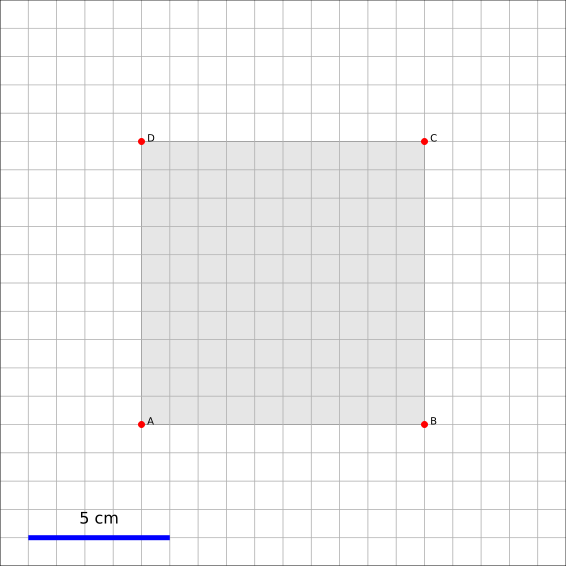
\includegraphics[width=0.6\textwidth]{../patterns/simple_scripts_0__FullSize}
\end{center}
\caption{Mon beau carré}
\label{fig:carre}
\end{figure}

Vous noterez en ligne (27) que l'ordre du dessin du polygone est définit A-B-C-D-A. On aurait pu mettre A-D-C-B-A pour un résultat identique à première vue. On parle ici d'un polygone fermé. l'ordre indiqué va permettre à la librairie graphique de tracer les segments dans l'ordre souhaité. On verra plus tard, à mesure que la forme du patron et donc de son contour se complexifie que cet ordre  est important et conditionne la façon dont on incluera une pince ou tracera une courbe.

\section{Dessines moi une pince}

Imaginons que nous allons transformer notre carré un peu pour en faire un demi-trapèze et lui ajouter une pince (Attention ça va faire jupe !). Les étapes sont les mêmes l'ajout de la pince se faisant évidemment après la définition des points du segment impacté par cet ajout.

\lstinputlisting[language=Python]{./sample/simple_scripts_1.py}

\begin{figure}
\begin{center}
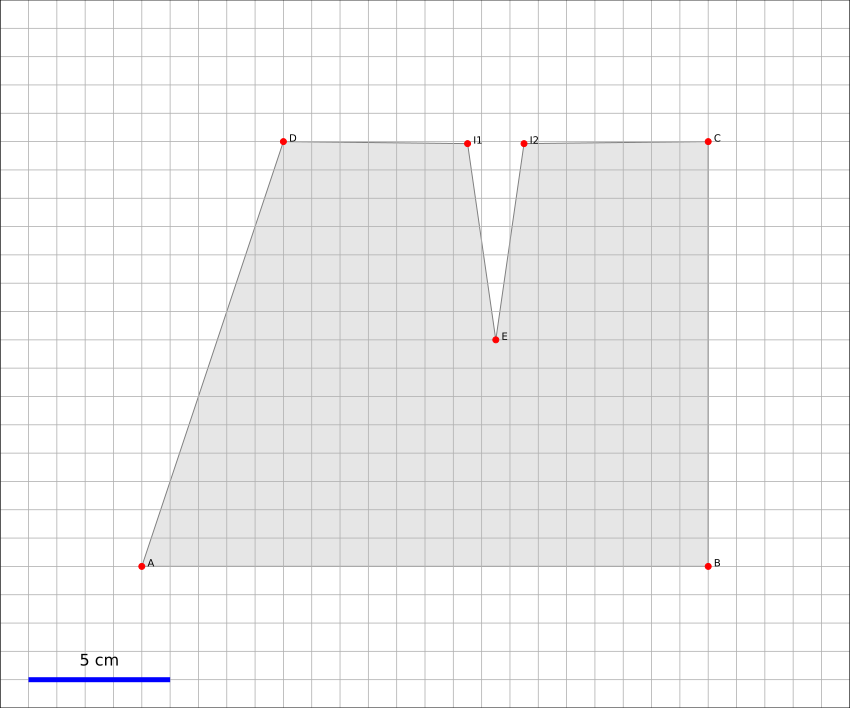
\includegraphics[width=0.6\textwidth]{../patterns/simple_scripts_1__FullSize}
\end{center}
\caption{Mon beau trapèze}
\label{fig:trapeze}
\end{figure}

Comme on le voit ici la création de la pince se fait en deux étapes. On définit la position du sommet de la pince (ligne 21) puis on appelle la fonction \texttt{add\_dart} en lui passant quatre arguments (ligne 22; il y en a plus que nous verrons plus tard) le sommet, les deux points définissant le segment qui doit être pincé et la largeur de la pince. la fonction renvoie la position des deux points qui, avec le sommet, constitueront la pince sur le patron.  Il ne reste alors plus qu'à intercaler les points de pince lors de la définition du trajet du tracé. La figure \ref{fig:trapeze} montre le résultat. Comment ça elle ne vous plait pas ma jupe ?

\section{Les annotations: légendes, marques et commentaires}

Un patron vient souvent accompagné de commentaires et de signes particulier comme l'indication du droit fil, les pliures et les crans de montages. Il est possible de les insérer sur votre patron à l'aide des commandes correspondantes comme le montre le script suivant et la figure qui l'accompagne (les commandes sont insérées dans le script précédent avant la commande \texttt{draw}).

\begin{lstlisting}[language=Python]
# add legends
myPattern.set_grainline(OP.Point([8,10]), 8, -np.pi/2)
myPattern.set_fold_line(C-[0,2], B+[0,2],'right')
myPattern.add_comment(OP.Point([12.5,15.5]),'TOP',0)
myPattern.add_comment(OP.Point([10,-0.5,]),'BOTTOM',0)


a = 70
myPattern.add_comment(OP.Point([2.8,8,]),'VV',a*np.pi/180) # workaround for notches
\end{lstlisting}


\begin{figure}
\begin{center}
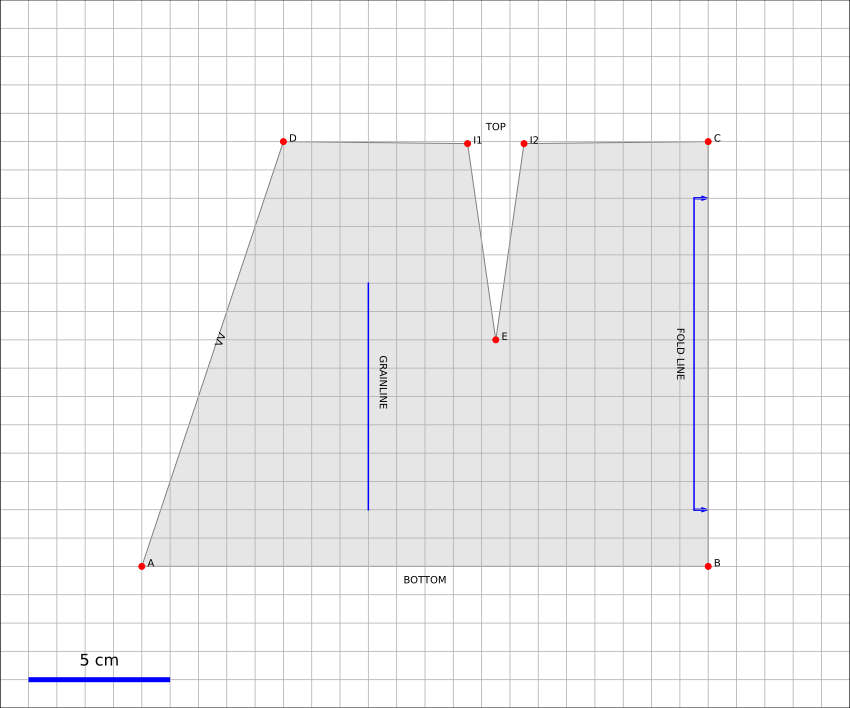
\includegraphics[width=0.6\textwidth]{../patterns/simple_scripts_2__FullSize}
\end{center}
\caption{Mon beau trapèze et ses annotations}
\label{fig:trapeze}
\end{figure}

On notera au passage qu'à l'heure actuelle un cran de montage se place comme un commentaire constitué de V en série.

\section{Les courbes et le pistolet}
Bien arrondissons les angles. Une jupe ce n'est pas juste un tour de taille mais aussi un tour de hanches et un arrondi sur le côté qui permet un passage doux de la taille à la hanche justement. Nous verrons à la section suivante l'utilisation des mensurations mais pour l'heure ajoutons une hanche «au hasard» et jouons sur la courbe latérale afin de comprendre de quoi il retourne.

\lstinputlisting[language=Python]{./sample/simple_scripts_2-2.py}

\begin{figure}
\begin{center}
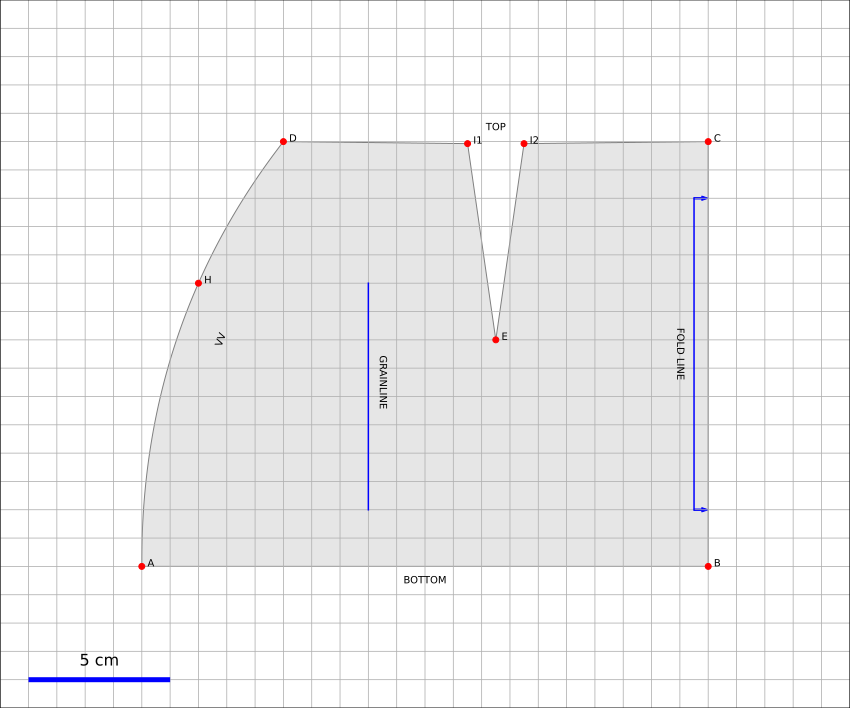
\includegraphics[width=0.6\textwidth]{../patterns/simple_scripts_2-2__FullSize}
\end{center}
\caption{Ma belle jupe}
\label{fig:trapeze}
\end{figure}

Les lignes nouvelles sont les 25,29,39 et 42. La 25 donne la déclaration du point de hanche H (hip en anglais). La 39 déclare ce point en l'ajoutant au dictionnaire de points. Ces deux instructions ont déjà été vues. La nouveauté est dans la ligne 39. On appelle la méthode \texttt{pistolet} de l'objet \texttt{pattern}. Cette méthode va tracer une courbe passant par les trois points D,H,A. l'ordre est important car la courbe est en fait approximée par une succession de 30 points qui sont renvoyés par le programme sous la forme d'une liste ici curve\_points. Le premier argument retourné correspond à la distance cumulée le long de la courbe et est surtout utile pour les calculs de manches. nos points iront donc de D à A en passant par H. cet ordre correspond à l'ordre dans lequel est défini le polygone du pourtour de la jupe (rappelez-vous ce que nous avons écrit lors de l'établissement de notre premier patron)). Ce dernier est définit en ligne 42 où l'on voit la façon dont on introduit la courbe

Notons qu'il faut au moins trois points pour tracer une courbe et l'ordre de la courbe est au maximum egal au nombre de points moins 1. Ici l'ordre sera de 3-1 = 2 au maximum. Ces courbes ne sont pas de simples polynomes mais des b-splines qui permettent de remplacer de façon très satisfaisante les clotoïdes ou courbes d'Euler ou encore «French curves» des pistolets traditionnels. De façon générale les splines d'ordre 2 suffisent pour tracer les pinces de côté des jupes ou les courbes de tailles, les splines d'ordre 3 sont nécessaires pour les têtes de manches qui présentent des points d'inflexions et certaines courbes de pantalon. Les splines d'ordre supérieur sont à peu de choses près inutiles en coupe à plat.




\section{Utiliser des sous-patrons}
Il est fréquent de créer un patron à partir de plusieurs bases différentes, buste et pantalon pour les salopettes par, buste et jupe pour certaines robes, ou encore buste, manche, col et manchette pour une chemise\footnote{On verra cependant dans ce dernier cas que la manche est intrinsèquement liée au buste. Elle vient «après» le dessin du buste}.

la classe \texttt{pattern} peut contenir d'autres \texttt{pattern} qui sont enregistrées dans la liste de patrons \texttt{pattern\_list}. Nous allons reprendre notre patron de jupe et le copier trois fois en utilisant des propriétés de translation et de rotation et de copie de la classe \texttt{pattern}.

\lstinputlisting[language=Python]{./sample/simple_scripts_3.py}


\begin{figure}
\begin{center}
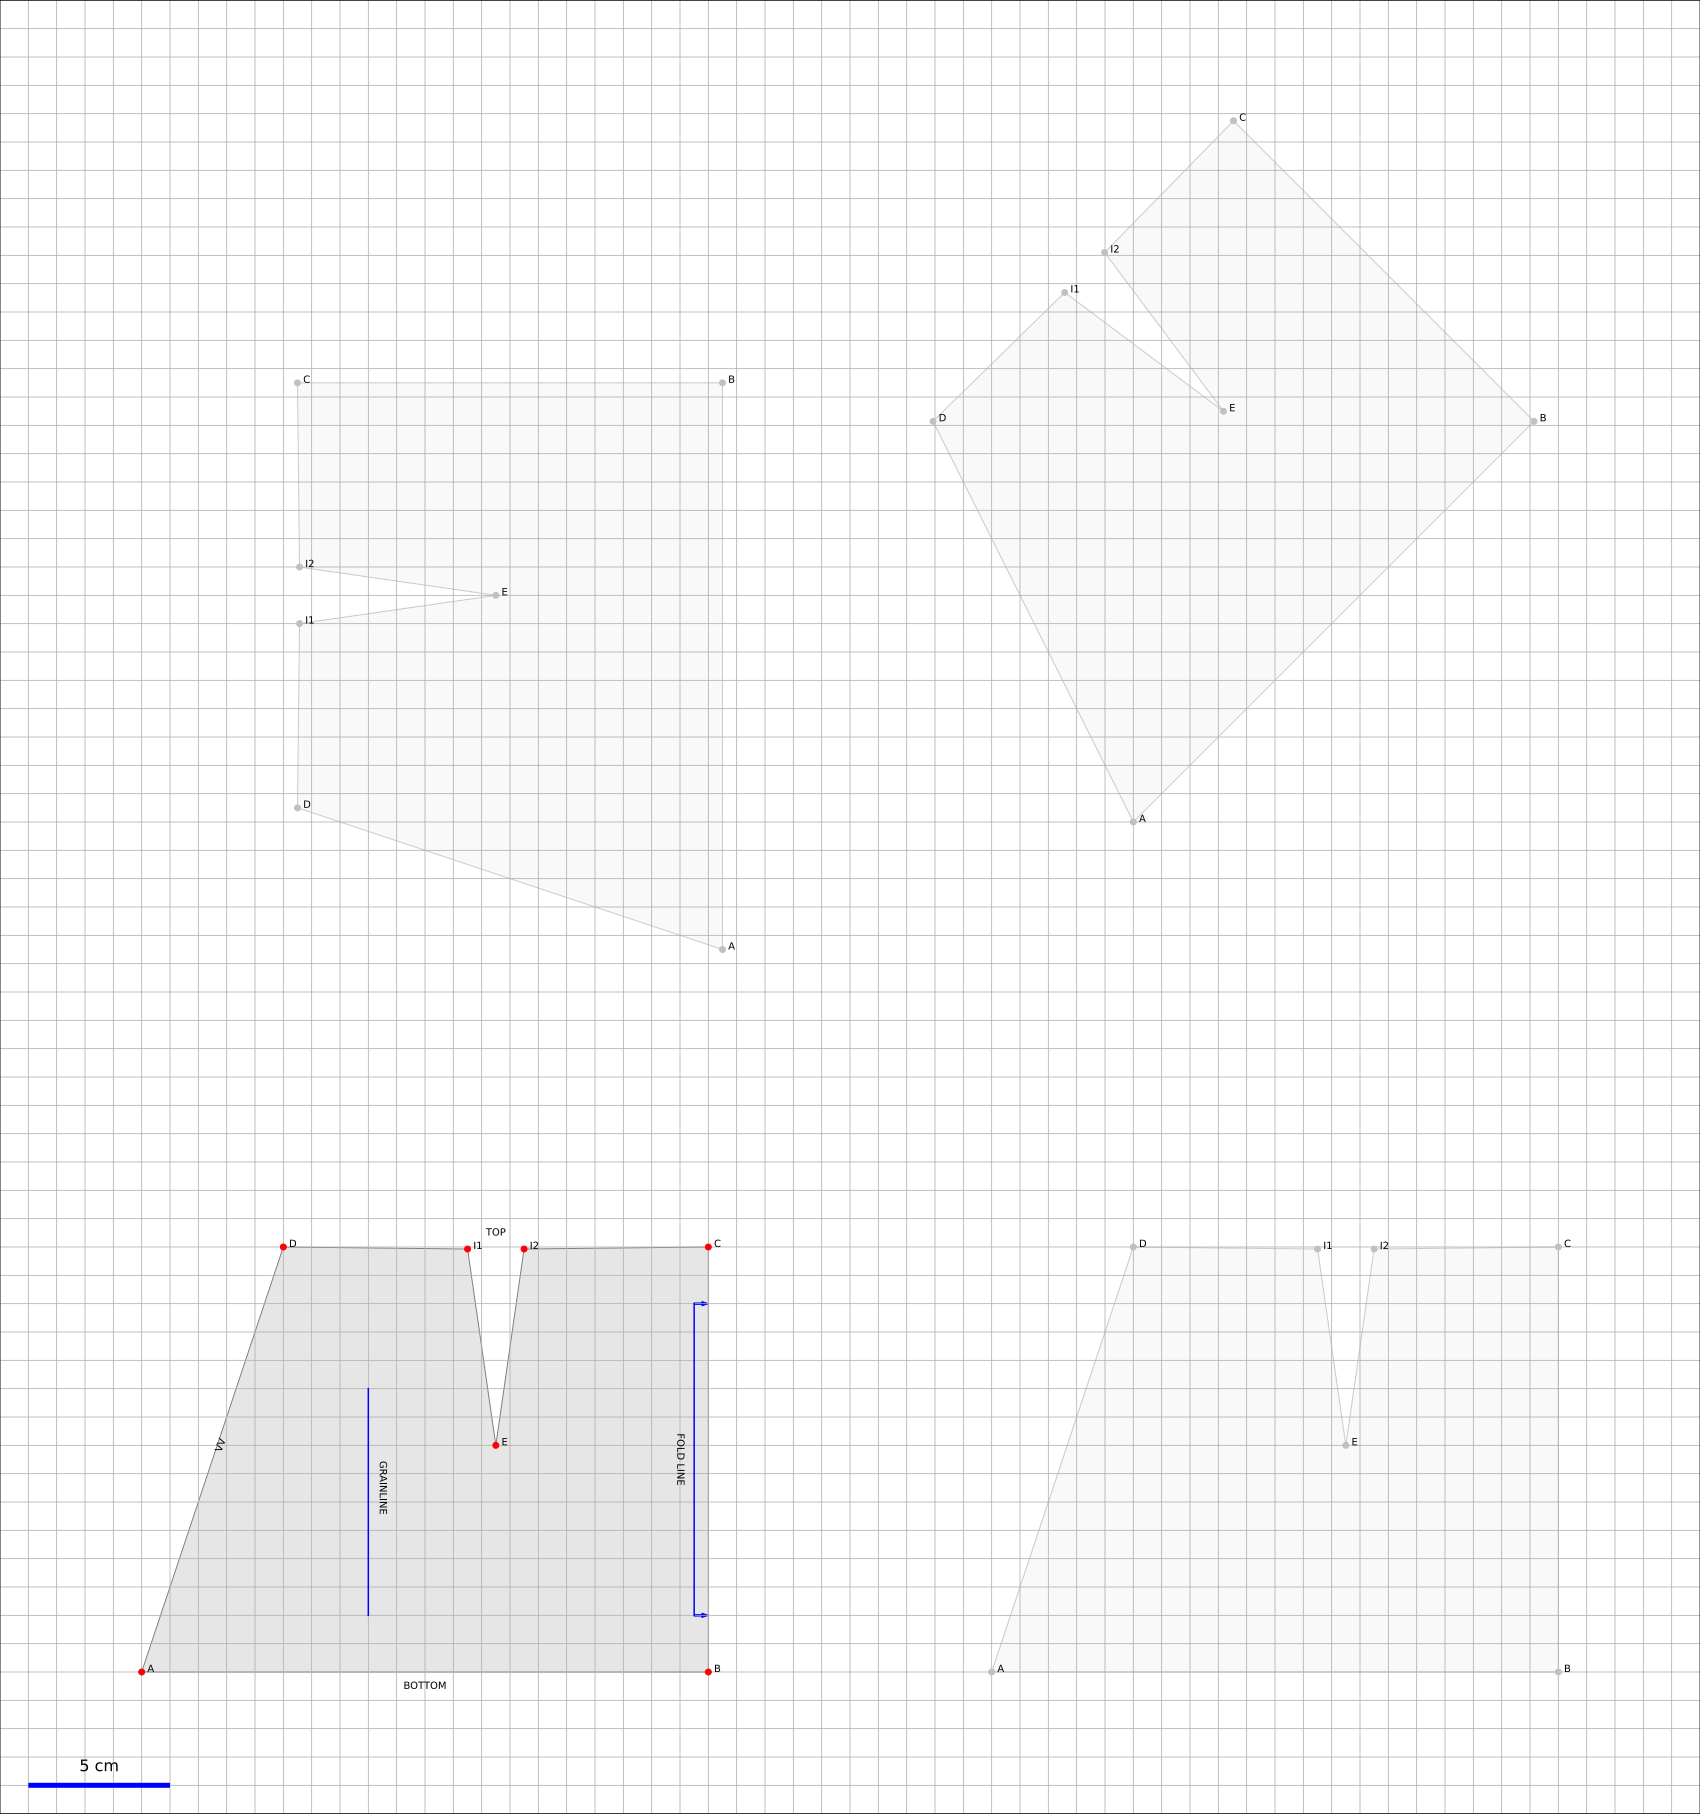
\includegraphics[width=0.6\textwidth]{../patterns/simple_scripts_3__FullSize}
\end{center}
\caption{Patron composite: mon beau trapèze et ses trois avatars}
\label{fig:trapeze}
\end{figure}

La partie qui nous intéresse ici débute à la ligne 47. Il s'agit de copier le patron de départ dans P2, P3 et P4 puis de le translater ou lui faire faire une rotation par rapport à un de ses points. Enfin le patron est ajouter à la liste de sous-patrons de myPattern. Pour le dessin on commence par dessiner les sous patrons sur une même figure puis on dessine le patron principal et on ajoute les légendes. Enfin lors du dessin de sous-patrons vous pouvez activer l'overlay qui les dessine avec un remplissage plus léger dans le but de pouvoir dessiner les altérations par dessus ultérieurement dans la teinte de gris classique.


\section{Utiliser des mensurations}

Bespoke my dear ! l'intérêt de la classe \texttt{pattern} c'est qu'elle peut faire appel à des mensurations c'est à dire un ensemble de mesures corporelles. Il en existe deux types. Les mesures standards correspondent à des moyennes statistiques sur une population d'une certaine taille ou d'un certain âge et d'un sexe donné. Elles varient avec le temps et suivant les auteurs car les populations à l'origine de ces jeux de données varient elles aussi. Les mesures individuelles (ou sur-mesure ou encore bespoke) correspondent aux mesures prises sur une personne précise. Elles ne correspondent qu'à elle et n'ont aucune utilité pour les autres mais elles correspondent au mieux à cette personne.
En utilisant des mensurations standards ou sur-mesure on peut ainsi adapter les patrons pour un publique divers ou ciblé.

Les mesures sont enregistrées dans une base sqlite3 à laquelle accède la classe \texttt{pattern}. Lors de la création de l'objet patron on peut appeler une des mesures enregistrées dans la base. Par défaut la classe est instanciée en chargeant les mensurations féminine de 38 données par Gilewska \cite{Gilewska1}. Ces mensurations sont chargées dans un dictionnaire nommé \texttt{m}.

Maintenant que vous savez tout faire le plus simple consiste à faire une vrai jupe. Nous allons donc tracer le patron d'une demi-jupe avant d'une fille de 8 ans selon la méthode de Jacqueline Chiappetta \cite{Chiappetta1999}.

\lstinputlisting[language=Python]{./sample/simple_scripts_4.py}


\begin{figure}[tb]
\begin{center}
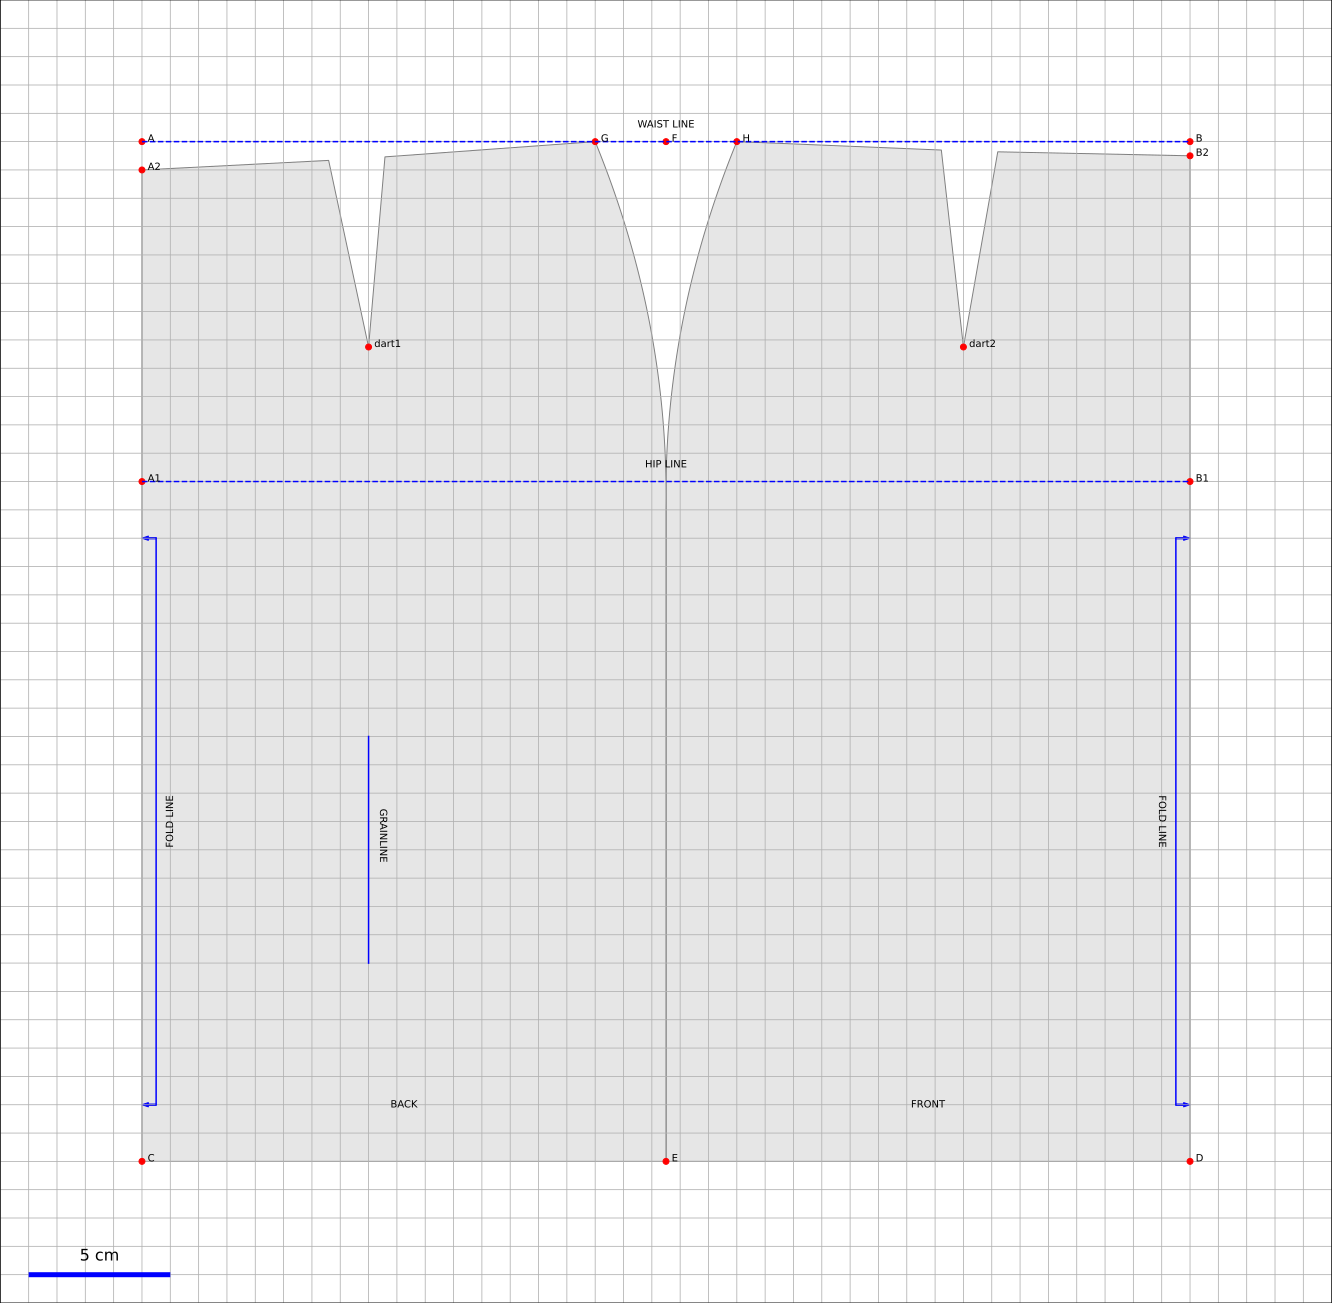
\includegraphics[width=0.8\textwidth]{../patterns/simple_scripts_4__FullSize}
\end{center}
\caption{Jupe droite, 8 ans, avec pinces, méthode de Jacqueline Chiappetta}
\label{fig:trapeze}
\end{figure}

Quelques commentaires s'imposent. De façon générale et même si de nombreuses variations existent les patrons de vêtements sont présentés avec une partie frontale et une partie dorsale. Notre jupe aura donc une patron pour le devant (front) et le dos (back). Ceci explique la présence de deux dicionnaires et de deux listes de points pour le polygone de chacun des élements du patron (lignes 55 à 72).

Notez la façon dont on appel les mesures \texttt{mfs.m["hauteur\_taille\_genou"]} par exemple qui renvoie la hauteur taille-genou correspondant à la taille appelée lors de la création du patron \texttt{mfs}. La liste des mesures disponibles en fonction des tailles et des sources est discutée plus en détail au \S\ref{par:tailles}

Un vêtement est dessiné avec une aisance (ease) qui doit être donnée en début de dessin. Ici on prend une aisance de 8cm pour l'ensemble du patron (17). La profondeur de pince dépend souvent aussi de la taille et de l'âge du modèle. Pour 8 ans chez Chiappetta \cite{Chiappetta1999} on a une pince de 7.25 cm (16). Les lignes de 19 à 35 permettent de tracer les points principaux du tracé de la jupe. Les lignes 39 et 41 permettent de créer deux points qui n'apparaîtront pas mais sont important. il s'agit de points de contrôle pour le tracé de la courbe du côté. En effet la courbe va de la ligne de taille à la ligne de hanche. Chiappetta ne  prend pas la peine de dire comment faire car avec un pistolet c'est évident (essayez pour voir et vous comprendrez). Par contre pour un spline et de façon générale en informatique il faut tout expliquer au programme qui ne fait que ce qu'on lui dit de faire (ce n'est pas un réseau de neurones !). Il faut donc définir le point milieu de la ligne de hanche (39) puis un point situé 1 cm au dessus qui permettra un tombé vertical de la courbe au point de hanches (41). Ces deux points ajoutés au point de taille H ou G suffisent à tracer une courbe pour le demi-devant et le demi-dos (43-46). La suite ne pose aucun problème maintenant: ajout des pinces, enregistrement des points et des positions qui définissent chaque polygone de demi-jupe, ajout des commentaires  et enfin dessin ! Ce patron peut-être imprimé en taille réelle et directement utilisé pour une jupe droite d'une fille de 8 ans. Manque juste la ceinture  que vous pourriez réaliser très facilement maintenant (on y viendra plus tard rassurez-vous) !


\chapter{Pour aller plus loin}

\section{Les tailles}
\label{par:tailles}
Le tableau \ref{tab:meas_sum} recense l'état des mesures que contient la base sql d'OpenPattern, sans compter les quelques mesures personnelles que j'ai prises sur mes proches.

\begin{table}[htb]
\begin{center}
\begin{tabular}{llcccl} \hline
Source & Genre & Taille min. & Taille max. & Mesures & Code\\ \hline
Gilewska & Femmes & 34 & 48 & 25 &  W34G\\
Gilewska & Hommes & 36 & 54 & 24 & M36G\\
Donnanno & Femmes & 40 & 50 & 21 & W40D\\
Donnanno & Hommes & 44 & 54 & 19 & M44D\\
Wargnier & Hommes & 38 & 48 & 25 & M38W\\
Chiappetta & Filles & 2 ans & 16 ans &23& W3C\\
Chiappetta & Garçons & 6 ans & 16 ans &20& G6C\\ \hline
\end{tabular}
\end{center}
\label{tab:meas_sum}
\caption{Tailles disponibles dans la base measurements. Le code donné en exemple correspond au code d'appel de la taille minimum.}
\end{table}

Notons que la distinction garçon, homme n'est pas anodine. En effet si les effets de la puberté sur les filles sont connus et aboutissent notamment à l'usage  des pinces de buste et de taille, les patrons de bases sans pinces ne changent pratiquement pas. Chez les hommes la puberté produit une inversion de la forme du buste. Le tour de poitrine d'un garçon est en effet plus petit que  son tour de bassin à l'instar d'une femme. De ce point de vue, important pour le dessin d'un patron, le garçon et la fille sont de morphologies proches et plus proche de la femme que de l'homme. La puberté inverse la situation chez l'homme dont le tour de poitrine devient plus grand que son tour de bassin. Ce changement influence de façon nette le traçage du patron masculin et ce qu'on y projette dans tous les sens du terme même si de façon étonnante ceci n'est jamais discuté.

J'ai recensé 51 mesures différentes chez mes sources. La répartition de ces différentes mesures en fonction des sources (tableau~\ref{tab:meas_det}) donne la mesure (:=)) des ennuis à venir. Chacun utilise un jeu de mesures communes mais brode en ajoutant ou pas des mesures différentes. Cela posera problème par exemple pour le tracé des épaules de l'homme qui présente des incohérence suivant les auteurs ou autrices. De façon générale l'homme est moins bien traité que la femme dans ces ouvrages (à l'exception des garçons de Chiappetta), probablement à cause du marché restreint qu'il représente et du moindre intérêt de son vestiraire (chemise, veste, pantalon pour faire simple). De fait ça part dans tous les sens chez les hommes... le plus gros écart sépare ceux qui mesurent la largeur des épaules et ceux qui mesurent la longueur des épaules. Quelques un mesurent les deux mais c'est plus rare. On notera que les mesures type varient d'un livre à l'autre. Pas toujours de mesure du tour de bras, du tour de jaret, du tour de cuisse.

Enfin pour ne rien gâcher les correspondances de tailles varient d'un pays à l'autre donc un 38 de Gilewska n'est pas un 38 de Donnanno... Officiellement il faut rajouter 4 aux tailles italiennes pour retrouver, approximativement, la taille française. Un 36 de Gilewska correspond donc à un 40 de Donnanno. Sauf que dans les fait quand on compare les valeurs on est plutôt sur une différence de 2 (un 38 Gilewska correspondant à un 40 Donnanno).

\begin{table}
\begin{center}
\begin{tabular}{lccccccc} \hline
Mesures & \multicolumn{2}{c}{Gilewska} & \multicolumn{2}{c}{Donnanno} & Wargnier & \multicolumn{2}{c}{Chiappetta}\\
& F & H & F & H & H & F & G\\  \hline
carrure devant&&&X&&&&\\ \hline
carrure\_devant&X&X&&&X&X&\\ \hline
carrure\_dos&X&X&X&&X&X&X\\ \hline
cheville\_terre&&&&&&X&X\\ \hline
crane&&&&&&X&X\\ \hline
ecart\_poitrine&X&&X&&&&\\ \hline
encolure\_dos&&&X&&&&\\ \hline
enfourchure&&&&&X&&\\ \hline
entrejambe&&X&&&X&&\\ \hline
entrejambe\_terre&&&&&&&X\\ \hline
fourche&X&&&&&&\\ \hline
genou\_terre&&&&&&&X\\ \hline
hauteur\_bassin&X&X&X&X&X&X&\\ \hline
hauteur\_carrure&X&&&&&&\\ \hline
hauteur\_corps&&&&&X&&\\ \hline
hauteur\_coude&X&X&&X&&X&X\\ \hline
hauteur\_emmanchure&X&&&&&&\\ \hline
hauteur\_petites\_hanches&X&&&&&&\\ \hline
hauteur\_poitrine&X&&&&&&\\ \hline
hauteur\_taille\_genou&X&&X&X&X&X&\\ \hline
hauteur\_taille\_terre&&&X&&X&&\\ \hline
hauteur\_tete&&&&&X&&\\ \hline
largeur\_encolure&X&&&&&&\\ \hline
largeur\_epaule&&X&&X&&&\\ \hline
largeur\_secteur&&&&X&&&\\ \hline
longueur\_col\_devant&X&&&&&&\\ \hline
longueur\_col\_dos&X&&&&&&\\ \hline
longueur\_devant&X&X&X&X&X&X&\\ \hline
longueur\_devant\_7c&&&&&X&&\\ \hline
longueur\_dos&X&X&X&X&X&X&X\\ \hline
longueur\_emmanchure\_devant&X&&&X&&&\\ \hline
longueur\_emmanchure\_dos&X&&&X&&&\\ \hline
longueur\_epaule&X&X&X&X&X&X&X\\ \hline
longueur\_manche&X&X&X&X&X&X&X\\ \hline
longueur\_taille\_terre&X&X&&X&&X&\\ \hline
montant&X&X&X&X&X&X&X\\ \hline
profondeur\_emmanchure&X&&&X&&&\\ \hline
profondeur\_encolure\_devant&X&&&&&&\\ \hline
profondeur\_encolure\_dos&X&&&&&&\\ \hline
profondeur\_poitrine&&&X&&&&\\ \hline
stature&&&X&X&&&\\ \hline
tour\_bassin&X&X&X&X&X&X&X\\ \hline
tour\_bras&X&X&X&&&X&X\\ \hline
tour\_cheville&X&&&&&X&X\\ \hline
tour\_cou&&&X&&&&\\ \hline
tour\_cuisse&X&X&&&X&&\\ \hline
tour\_encolure&X&X&&X&X&X&X\\ \hline
tour\_genou&X&&&&&X&X\\ \hline
tour\_jarret&&&&&X&&\\ \hline
tour\_mollet&&&&&X&X&X\\ \hline
tour\_petites\_hanches&X&&&&&&\\ \hline
tour\_poignet&X&X&X&&X&X&X\\ \hline
tour\_poitrine&X&X&X&X&X&X&X\\ \hline
tour\_poitrine\_haute&&&X&&&&\\ \hline
tour\_taille&X&X&X&X&X&X&X\\ \hline
tour\_tete&&&&&X&&\\ \hline
\end{tabular}
\end{center}
\label{tab:meas_det}
\caption{Répartition des mesures par source}
\end{table}




\section{Déplier un patron}
Déplier un patron peut-être utile pour des transformations. En effet très souvent les demi patrons de buste, de jupe et de robes sont au pli afin d'éviter des coutures inesthétiques au milieu (devant et dos). Lors des transformations par contre, comme pour transformer une jupe de base en jupe portefeuille par exemple, il peut être utile de travailler sur le patron déplié.   La méthode \texttt{unfold} permet cela. Sur le principe on fournit  un axe AB de symétrie, et pour chaque point du patron on cherche le point miroir. Ici cela est fait en deux temps: (1) projeter un point $O$ du patron sur la droite $(AB)$ pour obtenir le point $M$ et (2) chercher le point $O'$ qui se trouve à deux fois la distance de projection soit
$$\overrightarrow{OO'} = 2\overrightarrow{OM}.$$

Le script suivant montre comment procéder et la figure~\ref{fig:unfold} donne le résultat

\lstinputlisting[language=Python]{./sample/simple_scripts_5.py}


\begin{figure}
\begin{center}
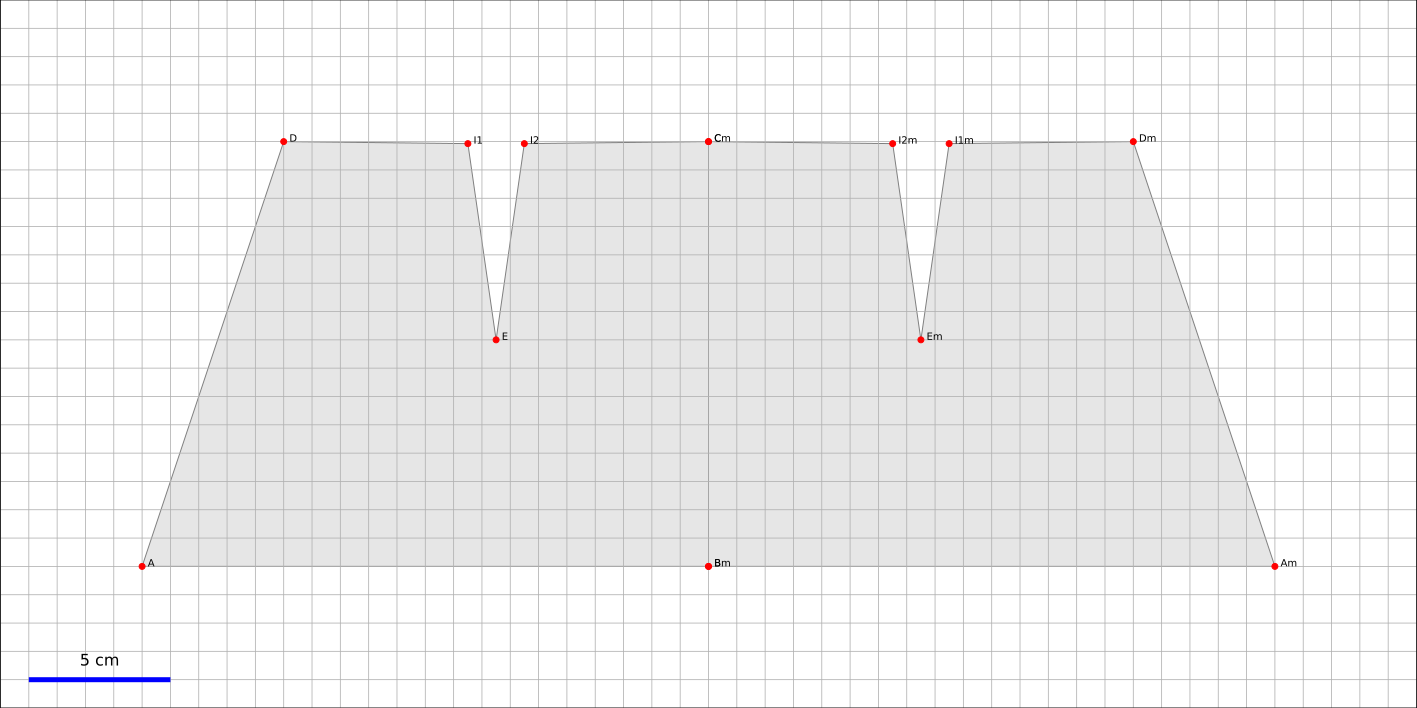
\includegraphics[width=0.6\textwidth]{../patterns/simple_scripts_5__FullSize}
\end{center}
\caption{Mon beau trapèze déplié}
\label{fig:unfold}
\end{figure}





\chapter{Commentaires}


\section{Shoulder line}

Pour les femmes de style G, la  onstruction des épaules repose sur des angles fixes. Pour les hommes de style G, cela dépend des distances par rapport à la ligne des épaules comme podonc ur le style D. Pourquoi ce changement? Cela pose un problème car, si l'on suit les instructions, l'épaule est plus longue que les mesures (si elles existent) et les épaules avant et arrière n'ont pas la même longueur. Dans le cas où la longueur d'épaule est donnée, la solution est alors d'ajuster la longueur d'épaule à la longueur mesurée à laquelle la ligne d'épaule a été établie (comme suggéré par Donnanno). J'ai donc ajouté un test pour l'existence d'une mesure de la vraie longueur des épaules Si tel est le cas, la longueur de l'épaule est ajustée pour s'adapter aux mesures. Notons en outre que les largeurs d'épaules correspondent chez G homme si on ne baisse pas l'épaule devant de 7cm mais de 5 (comme chez Donnanno).


Pour les adolescents (garçons) de style C, l'épaule repose sur deux angles différents pour le dos (22 $ ^ o $) et le devant (25 $ ^ o $).



\section{Armhole and collar}

à noter que, encore une fois, pour l'homme tout est un peu fait par dessus
la jambe. Ok des chemises des pantalons et des costumes c'est pas
folichon mais quand même !

Donnano:  pour les femmes le buste de base présente un problème d'ajustement car il ne
fournit pas de points de contrôles. J'ai repris ceux de Gilweska.

Pour l'hommes: pas de buste de base j'en au  créé un à partir de la chemise de base.
relativement simple à faire. Par contre problème (toujours) pour les
longueurs d'épaule. La largeur d'épaule est donnée mais pas la
longueur (qui d'ailleurs n'est que très rarement donnée pour les
hommes). or on demande la longueur d'épaule (j'adore le e.g. 17cm mis
dans l'exemple dont on ne sait pas d'où il sort)

Gilewska : pour le buste homme j'ai ajouté  deux points de contrôle
en base de manche  afin d'assurer la platitude d'emmanchure. Sinon les
spleen ne veulent pas faire comme le perroquet.


Chiappetta pour adolescents: (figure ~ \ ref {fig: CB14}) n'utilise qu'une seule mesure de carrure celle du dos. Pour les adolescents de plus de 10 ans, elle récupère juste deux cm de carrure mesurés au dos pour le devant. Le collier arrière a besoin d'un deuxième point de contrôle près de la ligne de pliage pour assurer la planéité de la cannelure.

Pour l'enfant Chiapetta changer l'angle, la longueur des points de contrôle et la carrure devant. de 2 à 8 ans les angles d'épaule devant et derrière sont les même, les longueurs plus petites et la carrure devant et dos sont les mêmes.

L'emmanchure et l'encolure sont faites avec des splines de second ordre. J'ai fini par jouer sur le fit des splines et les points de contrôle. À développer.

Bon mais comme d'hab Chiapetta ça à l'air un peu ringard sur les bords mais ça marche tout seul. je pense que je vais investir dans
les bouquins adultes notamment pour l'homme...


\section{Manches}
Gilewska: Aucune indication pour le bas de manche de base il faut donc
se débrouiller seul avec le tour de poignet...

Les splines ici sont du troisième ordre car il y a un point d'inflexion.


De façon générale je trouve que les bustes hommes ne sont pas très ressemblant aux dessins des livres et je suis dubitatif car le programme reproduit exactement les instruction sauf quand c'est problématique de façon évidente (genre les largeur d'épaules de Donnanno).


\section{Collars}
Styles available from Gilewska men: Officer and OnePiece (for one piece collar)

\begin{figure}
\begin{center}
\includegraphics[width=0.48\textwidth]{../patterns/collar_Gilewska_OnePiece_M44G_FullSize.pdf}
\includegraphics[width=0.48\textwidth]{../patterns/collar_Gilewska_Officer_M44G_FullSize.pdf}
\end{center}
\caption{Collar styles}
\end{figure}


\section{Cuffs}
Styles availabel from Gilewska men : Simple and French

\begin{figure}
\begin{center}
\includegraphics[width=0.48\textwidth]{../patterns/cuff_Gilewska_Simple_M44G_FullSize.pdf}
\includegraphics[width=0.48\textwidth]{../patterns/cuff_Gilewska_French_M44G_FullSize.pdf}
\end{center}
\caption{Cuff styles}
\end{figure}

\section{Trousers}


\subsection{Pants Block}

Incohérence du modèle chez Donnanno. La mesure de la ceinture est
$$AV = Hip + 6.$$
Or la somme
$$ceinture avant + ceinture arriere = Hip +2.$$
Donanno indique qu'il faut séparer les patrons avant et arrière de 6cm soit
$$ceinture avant + ceinture arriere + 6 = Hip +8 = AV,$$
d'où l'incohérence.

\section{skirts}

jupe de base une pince. position de la pince.

Chiappetta: à mi-distance jusqu'à 12 ans. 2 pince au 1/3 et 2/3 de distance pour 14 et 16 car l'écart entre taille est bassin est trop grand pour être absorbé en une seule pince. Chiappetta rappelle qu'avant 10 ans on ne met que rarement les pinces car les jupes sont presque systématiquement élastiquées. Est-ce encore vrai ?

Donnanno: à une distance d'1/2 bust point --- non défini mais qu'on imaginera être le téton--- que je comprends comme le demi écart poitrine.

Gilewska: confirme l'utilisation du 1/2 écart poitrine. Si la différence taille/bassin est trop importante alors Gilewska recommande deux pinces devant une au 1/2 écart poitrine et une à mi distance entre la première pince et la pince de côté (le côté de fait). utlise une pince de milieu dos

la bande de taille chez Donnanno est donnée à 5cm

\bibliographystyle{plain}
\bibliography{OpenPattern.bib}

\end{document}
